\section{Distributed Hash Tables}
The implemented distributed hash table has it's entries distributed among several active objects. The data is therefor stored in many actors but not on different machines. The programmer can change how the hash tables distribute data but a standard is provided. Looking in from the outside interacting with distributed hash tables is very similar to how one would interact with any normal hash table. The method put(key,value) is used to insert values into the the distributed hash table and get(key) method is used to extract values. In the view of the programmer which worker hold specific values are not important and it all is calculated under the hood. 

\begin{lstlisting}
var ageTable = new Bighash[String,Int](StringID)
ageTable.put("Kent",19)
ageTable.put("Eric",21)
var ericAge = ageTable.get("Eric")
println(ericAge)
\end{lstlisting}

The Encore code above show the creation of a distributed hash table and usage of the put and get methods, this block of code will print 21 to the standard output. In the Implemented Encore library distributed hash tables is implemented by a class named Bighash. \\

\begin{figure}[h]
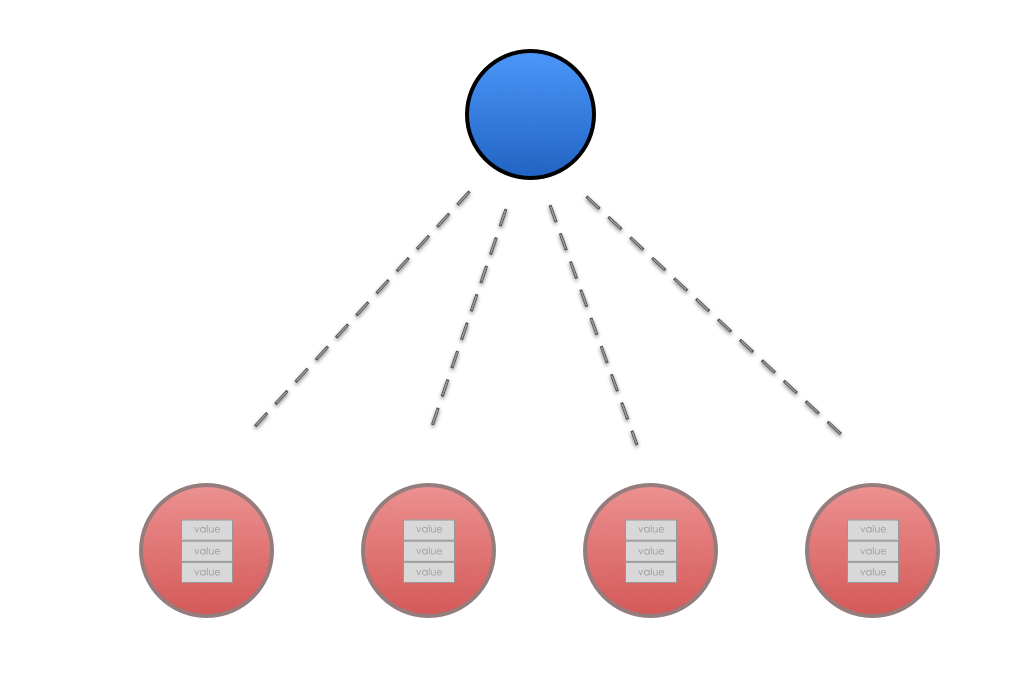
\includegraphics[width=12cm]{images/originalFigure}
Figure(2): Overview of a distributed hash table with one supervisor (blue) that hold references to four workers (red), each worker hold a number of hash-entries.
\end{figure}

\subsection{Structure}
At the lowest level there are a set of active object that each hold values owned by the distributed hash table, these active object is referred to as workers. There are also Supervisors, Supervisors exists in the top level and has pointer to all workers at the bottom level. Supervisors also hold all necessary information about the structure of the distributed hash table such as how many workers exist, how big they are and the hashing function used. The supervisor is also responsible for hashing the input key, the hashed key value is used to determine which worker should own specific values. Methods calls applied to the distributed hash table are first handled in a supervisor and then asynchronous calls is sent to the workers to preform the request to one or more values. Some method calls that only return information never need to access the bottom level because the supervisor hold all necessary information \\

\begin{lstlisting}
linear class Supervisor[sharable k,sharable v]
    var numOfWorkers: int
    var workers : [(Worker[k,v])]
    var workerSize : int
    var siphash: Siphash
    var hashFunction : k -> uint
\end{lstlisting}

The implemented Supervisor class, it's linear which means it can be consumed and passed to other active objects, sharable k and v are generic key and value types and sharable makes it possible to pass them to the bottom level.

\subsection{Functionality}
\subsubsection{Creating Reference}
To efficiently use a distributed data type of this kind the bottom level must be able to be accessed from more than one place. If all messages is sent to the original reference of the data type, it would be a bottleneck. The top level consist of of a class of type linear which means there can only be one reference to that object and it can be passed to other active object only by consuming it \cite{kappa}. Before the programmer consume the distributed hash table it can copied with the .copy method. Copy creates a new passive supervisor object with the same information but instead of creating new workers at the bottom level it holds references to the original ones. This copied supervisor can now be consumed instead of the original one and passed to other active objects and used just as the original. \\

\begin{figure}[h]
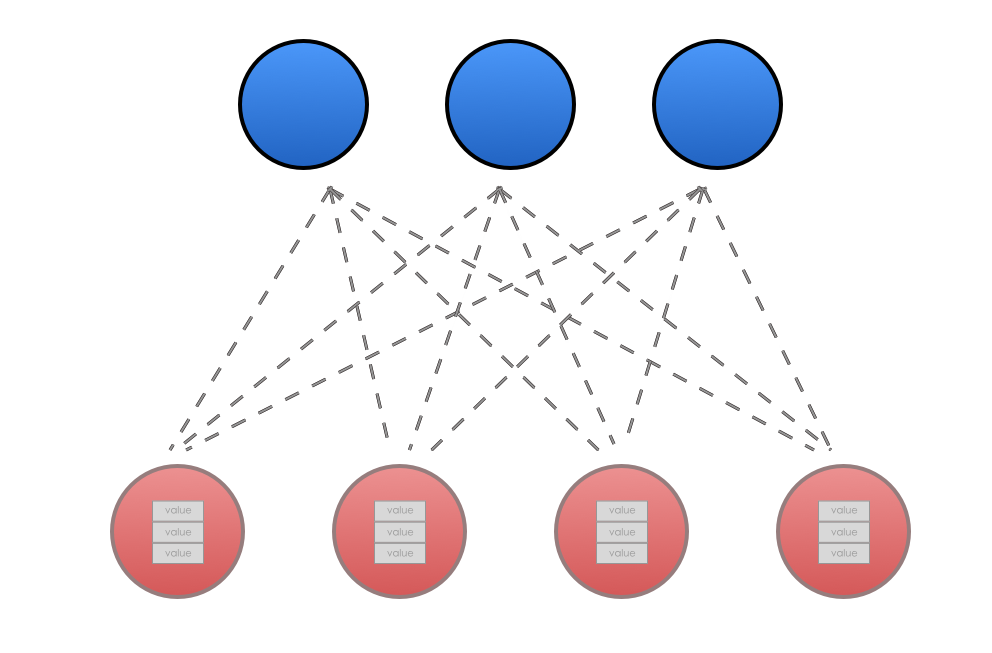
\includegraphics[width=12cm]{images/WithManySupr}
Figure (2). The original distributed hash tables have been copied 2 times and the bottom level has 3 supervisors sending messages to it. 
\end{figure}

Note that the bottleneck of only having one reference is gone. All the workers have it's own message queue and can therefor handle messages and run concurrently and be scheduled on different cores. The messages could also be sent from different active objects and therefor they too would be able to run on different cores.

\subsubsection{Rehashing}
As mention in the section Design Challenges, creating more references and supervisors result in some problems. If one supervisor wants to start rehashing and change structure of the distributed hash table it can send messages to all workers at the bottom level but the problem is that only that supervisor then has a correct view of how the hash tables currently is structured. One could stop message sending and try to update all reference, but this is not a simple solution. \\

The solution implemented into this library is that no references send rehash request, instead the individual worker at the bottom level rehash itself and double it size automatically when more then 75\% of the hash entries contain values. With this solution how big each worker is not visible from the top layer but it is not necessary, the real trade off is that after copying the data type the number of workers can not be changed. The gain with individual hashing is that if for some reason the distributed data type is not very even distributed, only the workers that needs to get bigger will increase in size.   

\begin{figure}[h]
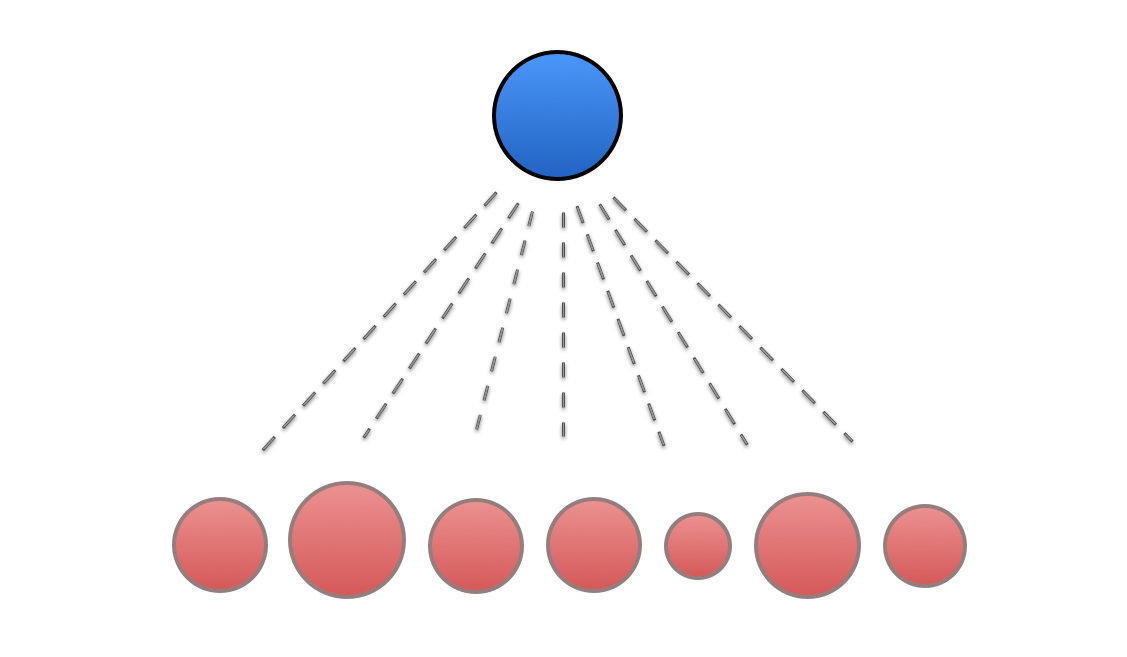
\includegraphics[width=12cm]{images/Resizing}
Figure (3). Each worker resize itself automatically if needed. To have very unevenly sized workers can slow down performance, it is however memory efficient to avoid having big workers with many empty hash-entries.
\end{figure}

\begin{lstlisting}
def resizeIfNeeded() : unit
    if (this.tableSize - this.filledEntries < this.tableSize/4) then
       this.rehash()
    end
end
\end{lstlisting}
This function checks if a worker is needed to be resized and rehashed, resizeIfNeeded() is run before inserting any value into a worker hash-entry.

\subsubsection{Working with Generic Types}
When implementing a hash table some unique identifier for each object that is used as a key is needed. In the Language Java every object has an unique id and that could be used but Encore do not provide such features. The id is needed to work both with user created classes and normal Encore data types. The idea is that when two string contains the same characters it should generate the same hash so no pointer value can be used. In the current implementation the problem is solved by asking the programmer to provide a function that transform the key value to a uint type, the uint is later used in the Siphash \cite{siphash}. For some basic types the implemented library provide hashing functions. A function of this type must be provided in the initializing of the distributed hash table, see code below for how one could creating a unique identifier for strings.

\begin{lstlisting}
EMBED
uint64_t strHash(char* input);
BODY
uint64_t strHash(char* input) {
    uint64_t hash = 5381;
    char *str = input;
    int c;

    while ((c = *str++))
        hash = ((hash << 5) + hash) + c;
    return hash;
}
END

fun stringID(s : String) : uint
    var ans = EMBED (uint) (uint64_t) strHash(#{s.getData()}); END
end
\end{lstlisting}
This example contains embed statements which allow you to write C code into Encore, the C algorithm used for hashing strings is called djb2 and was original implemented by Dan Bernstein \cite{string_hashing}. The Encore function StringID can be used in a distributed hash table where Strings are used as key values.

\subsubsection{Hashing Algorithm}
The key value hashed to the uint type from the user provided function is later hashed with an implementation of Siphash, the Siphash implementation was created by a previously bachelor worker \cite{lucas} on Uppsala University. Siphashes are optimized for short input's and was created to provide protection from hash-flooding \cite{siphash}. Siphashes will therefor create a very distributed hashing which is very important for a distributed hash tables to be efficient.

\subsubsection{Data Distribution}
When the final key value is hashed it is then used in an algorithm to calculate which worker that should own the corresponding value. The algorithm is simply the hashed key valued modulo number of workers, this result in a number which can be used as a worker id in the list with worker pointers.

\begin{lstlisting}
def put(key:k,value:v) : unit
    var hash = this.generateHash(key)
    var workerID = this.modulo(hash,this.numOfWorkers)
    this.workers(workerID) ! put(key,value,hash)
end
\end{lstlisting}
The is the part of put method that is in supervisors class, a message is sent the worker and it will store inserted key value pair as well as the hashed key value.

\subsubsection{Finding Hash-entries}
\subsubsection{List of Implemented methods}
\begin{center}
    \begin{tabular}{ | p{4cm} | p{10cm} |}
    \hline
    Method name and type: & Description: \\ \hline
    put(k,v) : unit & Stores value v at key k \\ \hline
    remove(k) : unit & Remove all values at key k \\ \hline
    get(k) : v & Returns first value at key k \\ \hline
    getMany([k]) : [v] & Returns a list with first value at each key k \\\hline
    keys() : [k] & Returns all keys \\ \hline
    elements() : [v] & Returns list of all values stored in the hash table \\ \hline
    contains(v) : bool & Returns true if value is stored in hash table \\ \hline
    clear() : unit & clears all hash entries in hash table \\ \hline
    extend(k,v) : unit & Extends a value for at key k \\ \hline
    extendAll(k,[v]) : unit & Extends values at key k \\ \hline
    getValues(key:k) : [v] & returns list of values at key k \\ \hline
    hashFunction() : f k-\> uint & Return the user user provider hash-function \\ \hline
     getSizing() : (int,int) & returns workers size and number of workers \\ \hline
     copy() : Bighash[k,v] & Returns a object with pointers to same hash-entries as the original\\ \hline
    putManyandBatch       (pairs:[(k,v)]) : unit & Sort pairs and send one messages with many pairs to workers \\ \hline
    \end{tabular}
\end{center}
\begin{center} Table 1. List of supported methods for the implemented distributed hash table \end{center}


\section{Distributed Arrays}
\subsection{First Prototype}
The distributed arrays was the first prototype to be implemented. Focus was later changed to the distributed hash tables which with the knowledge gain from the array implementation evolved to have more advanced functionality. They both are based on the same idea and much functionality are very similar. Here are some example how the distributed arrays are used. \subsection{Example Program}

\begin{lstlisting}
import Bigvar

class Main
    def main() : unit
        var people_array = [new Person("Josef",22),
                            new Person("Erik",23),
                            new Person("Sahand",17),
                            new Person("Joel",15),
                            new Person("Basse",23)]

        var people = new Bigvar[Person](people_array)
        var peopleOfAge = people.filter(fun(p:Person) => p.age > 18)
        peopleOfAge.update(fun(p:Person) => p.salary = salary*1.2)
        payments = peopleOfAge.map(fun(p:Person) => (p.salary,p.banknumber))        
    end
end
\end{lstlisting}

The variable people is a distributed array constructed from the people\_array variable. Person objects that are out of age are filtered out then the all remaining Persons their salary are increased by 20\%. A new distributed array payments is then created with tuples of peoples salary and bank numbers. Note the is only to showcase the use of the implementation, if this would be a real life applications bigger amount of data would be needed for it to have the possibility of being efficient program. 
